\chapter{Literature Review}
\label{ch3_lit_review}
OpenCL implementation Portable Computing Language (POCL) was studied as a part of the related work. It is portable and performance portable by virtue of a kernel compiler that can utilize the data parallelism of the program on different hardware architectures. Compiler transformations which produce work-group functions with multiple work items which can be parallelized are made by integrating the OpenCL implementation with LLVM compiler infrastructure. This newly implemented feature allows the kernels to be mapped to the parallel resources available on the different computing platforms
\cite{pocl}. The experiments conducted by Pekka, J. et al on multiple hardware platforms showed that POCL could successfully port OpenCL applications efficiently.\newline\newline
One main part of this project constitutes studying an OpenCL application based on Convolutional Neural Networks which recognizes digits from MNIST database. L. Yann et al talks about how multilayer neural networks trained with backpropagation algorithm make an efficient Gradient-Based learning technique. This was incorporated in his model of CNN, known as the LeNet-5 architecture. The authors state two main modules to split the neural networks system into for recognizing individual patterns. The first module is a feature extractor which changes the input patterns into low-dimensional vectors or short strings of symbols that allow easy comparison and are invariant to the distortions in the input patterns. The second module is a trainable classifier which is general-purpose 
\cite{cnn_yann1998}. L. Yann et al performs handwritten character recognition using several learning techniques on the benchmark dataset MNIST for handwritten digit recognition. Such an intricate convolutional neural network requires a large amount of computations, thereby requiring computational power for fast classifications.  \newline\newline
Instruction Set Architecture (ISA) refers to the set of instructions which a processor understands to execute an instruction. It is an interface between a computer’s software and hardware enabling high language code to execute on the machine. Different architectures use different bit sizes, number of operands for specific instruction types and endianness, which affect their performance.\newline\newline
Complex Instruction Set Computers (CISC) architecture, a predecessor of RISC, aimed to complete a task in as few lines of assembly code as possible. This, however, requires processor hardware capable of understanding complex instructions. RISC emphasizes on software and uses only simple instructions that can be executed in a single clock cycle. RISC architecture also reduces the load on hardware space, allowing more general purpose registers to be used
\cite{risc_vs_cisc}. Intel x86 has retained CISC architecture due to other technological advancements, but is still considered too complex for simple projects.\newline \newline
RISC-V was developed with the need to meet the case for a free and open source ISA. For over 30 years, no other ISA has been a successful stack ISA including CISC. In this regard, RISC-V is better than its predecessors by removing unnecessary features like shift and keeping necessary load/store byte capabilities
\cite{riscv_isa_free}.\newline \newline
Several implementations of processors based on modified RISC-V architecture are present. Few of them are studied in this section. Berkeley Out of Order Machine (BOOM) is a synthesizable, superscalar and out-of-order RISC-V core written in Chisel, the hardware construction language
\cite{boom_2015}. Chisel stands for Constructing Hardware in a Scala Embedded Language. It supports a multi-core processor system by replacing the in-order Rocket core with the out-of-order BOOM core. It provides support for floating point, atomics and page-based virtual memory.\newline \newline
PULPino is a Parallel Ultra Low Power Processor with a small single-core RISC-V System on Chip (SoC). It is a small part of PULP which is a huge energy efficient many-core SoC with multiple software framework support. PULPino focuses on simplicity by removing caches, memory hierarchy and DMA (Direct Memory Access). As seen from Figure \ref{fig:pulpino}, the processor has a single cycle access being directly connected to the instruction and data RAM. It consists an Advanced Peripheral Bus to allow easy addition of peripherals to the core. The Boot ROM loads the program from SPI Flash.\newline

\begin{figure}[h!]
  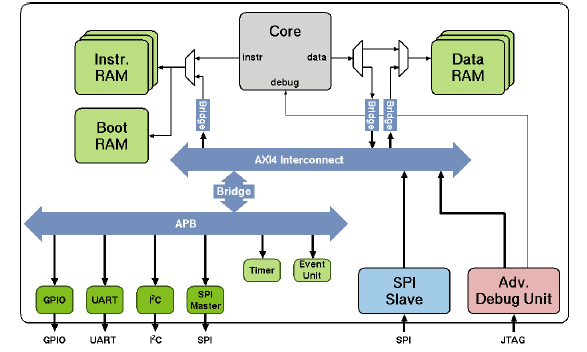
\includegraphics[width=\linewidth]{figures/pulpino.PNG}
  \caption{Architecture of PULPino single-core SoC
  \cite{pulpino}}
  \label{fig:pulpino}
\end{figure}
Sources related to existing implemented accelerators were studied to understand what is lacking in the current scenario. Hugo van der Wijst explains in his Master thesis the increasing need for better performing accelerators
\cite{thesis_2015}. He describes in detail his work on \textrho-VEX processor to create an accelerator, including the design considerations, implementation, experiments and results. As part of the implementation, a PCI Express communication is set up between the FPGA and the accelerator. \newline\newline 
The thesis continues to explain how \textrho-VEX can be used as an accelerator in an OpenCL runtime environment by computing various performance metrics through experiments. Open64 compiler is found to perform better than LLVM compiler. Open source implementation POCL was chosen as the OpenCL runtime for the new accelerator, with a device-layer added to support \textrho-VEX based accelerator. The execution time was improved by following techniques like reducing Instruction Count, Clock Cycles Per Instruction (CPI), memory stall cycles and clock cycle time. The parallel execution and data throughput was increased as well, to influence the execution time  \cite{thesis_2015}.\newline\newline
This project is different from the previous work, in the sense, it aims to develop a hypothetical engine with multiple CPUs, GPUs, and other co-processors acting as accelerators individually and combined in an overlay manner to provide a huge performance boost. Each core in the overlay would run RISC-V ISA and be capable of supporting OpenCL framework. This engine is different from the previous work in related areas, providing a new mega-accelerator platform to the computing world.
